\documentclass[a4paper,12pt]{report}

\usepackage[utf8]{inputenc}
\usepackage[T1]{fontenc}
\usepackage[french]{babel}
\usepackage[top=10mm,margin=20mm]{geometry}
\usepackage{graphicx}
\usepackage{caption}

\def\code#1{\texttt{#1}}

\begin{document}
  \begin{center}
   \Huge Rapport de projet
   \linebreak
   \linebreak
   \normalsize Mars Invaders - Architecture des Ordinateurs
   \linebreak
   \linebreak
   Gaëlle GIRARD - Lucas LETT
  \end{center}

\section*{Introduction et avis sur le sujet}
Ce sujet nous a paru vraiment intéressant. Il est vrai que le langage assembleur MIPS peut sembler un peu rébarbatif au premier abord, mais ce projet nous a permis de mieux le comprendre, en l'utilisant pour en faire quelque chose de ludique et motivant.\par
Au final, la réalisation de ce projet s'est révélée très enrichissante, et nous a presque donné l'envie de recoder d'autres jeux rétro (snake, Tetris ...) en MIPS pour s'amuser. 

\section*{Les différentes étapes de la réalisation}
Tout d’abord, nous avons tout deux dressé l’inventaire des différentes fonctions et des différentes données fournies dans le programme initial. Nous avons, pour chacune d’elles, identifié les registres d’entrée et de sortie, et avons décidé de garder la convention suivante pour mettre en œuvre nos fonctions : les registres \texttt{\$aX} servent de registres d’entrée, et les \texttt{\$vX} de registres de sortie.
Après avoir réussi à afficher les différents éléments à l’écran, tels que les aliens, les batiments et le joueur, nous avons commencé à nous répartir les différentes tâches à effectuer : la gestion des vitesses pour chacun de ces élements a été confiée à Lucas, tandis que l’implémentation de trois conditions de fin a été confiée à Gaëlle.\par
\vskip 0.75cm
Pour la gestion des vitesses, un système de modulo (fonction auxiliaire \texttt{modulo} a été codé, pour gérer de manière conditionnelle l'activation (ou non) du tir, du déplacement des aliens et du déplacement du shooter.
Du côté de l'implémentation des conditions de fin, la fonction \texttt{comptage\_aliens} a été ajoutée, pour permettre de vérifier plus simplement si tous les aliens ont été tués.\par
La gestion de la quatrième condition de fin, qui détecte si les aliens ont atteint le sol, a été confiée à Lucas. Après une première version fonctionnelle, une fonction auxiliaire a été ajoutée afin d’affiner la condition de fin. La mort des aliens situés dans les couches inférieurs va influencer la fonction précédente. Ainsi, le jeu ne se terminera pas si une ligne d’aliens vide atteint les bâtiments.\par
\vskip 0.75cm
Pendant ce temps, la mise en place d’un système de score, et de vies, a été réalisé par Gaëlle.
Le score se calcule comme tel : +100 points par alien tué, -1 point par tir.
Au niveau de l'implémentation des vies, une fonction teste si le joueur est bel et bien mort ou s'il lui reste une ou plusieurs vies. Au total, au début de la partie, il en possède 3.\par
\vskip 0.75cm
A ce stade, les fonctions permettant au jeu de réagir comme le sujet le demande ont été réalisées. Nous avons donc pris la liberté d'ajouter quelques fonctionnalités supplémentaires à notre Mars Invaders.
Par exemple, Lucas a programmé un système de cooldown qui agit entre chaque tirs, pour éviter l'effet ``mitraillette'' afin que le joueur ne gagne pas trop facilement.
Des couleurs ont aussi été ajoutées au jeu, notamment sur chaque ligne d'aliens ainsi que sur le shooter.
En particulier, nous avons ajouté un changement de couleur du shooter en fonction du nombre de vies restantes : moins il y en a, plus il sera rouge vif.\par
\vskip 0.75cm
Enfin, afin d’afficher du texte à l’écran, une fonction va permettre d’afficher des caractères en fonction d’un code héxa représentant le caractère, et à partir de l’adresse à laquelle nous voulons afficher le caractère. Realisée par Lucas, cette fonction a ensuite permis l’affichage d’une page de fin, indiquant si le joueur a gagné ou perdu, ainsi qu’une page de démarrage qui affiche le nom du jeu.
C'est Gaëlle qui s'est occupée de la gestion de l'affichage du score sur l'écran final.
Une fonction \texttt{afficher\_score} a été implémentée. Son rôle est d'isoler chaque caractère composant le score final au moyens de soustractions successives, puis de les afficher à l'écran lorsqu'on a gagné ou perdu.\par

\section*{Problèmes rencontrés}

Au final, les problèmes auxquels nous avons pu être confrontés étaient plus souvent relatifs au game design ainsi qu'aux mécaniques de jeu, plutôt qu'à la programmation en elle-même. En effet, même si le langage assembleur MIPS nécéssite un certain temps d'adaptation et de compréhension (notamment pour la gestion de la pile ainsi que pour les affectations de valeurs ou d'adresses (on ne compte plus les \texttt{li} au lieu de \texttt{la} et inversement ...), la prise en main se fait quand même relativement facilement.\par
\vskip 0.75cm
Le game design, lui, requiert une réelle réflexion: comment doser la vitesse de tir pour que le jeu ne soit ni trop facile, ni trop difficile ? À quelle vitesse régler les déplacement des aliens ? Comment choisir une charte graphique qui ne soit pas trop désagréable à l'oeil ? Comment établir un système de score équitable ?
Autant de questions dont le joueur n'a généralement pas conscience, mais dont on découvre l'importance lorsqu'on se trouve confronté à la conception soi-même.\par

\vskip 3cm
\begin{figure}[h!]
  \centering
  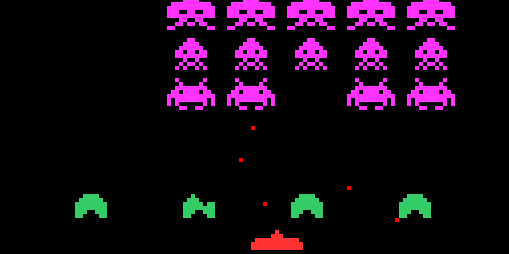
\includegraphics[scale=0.6]{invader}
  \caption*{La bataille fait rage ...}
\end{figure}


\end{document}